\documentclass[a4paper]{jpconf}
\usepackage{graphicx}
\begin{document}
\title{PyFAI, a versatile library for azimuthal regrouping}

\author{J\'er\^ome Kieffer, Dimitris Karkoulis}

\address{European Synchrotron Radiation Facility; 6 rue Jules Horowitz;
38043 Grenoble; France}

\ead{jerome.kieffer@esrf.fr}

\begin{abstract}
Area ($2d$-) detector like CCD or pixel detectors have replaced punctual detector
over the 15 last years in diffraction (both in WAXS, SAXS and single crystal
diffraction). Those detectors with wide sensitive area have micron-sized spatial 
resolution and provide millions of pixels. PyFAI was designed to reduce SAXS and
WAXS images taken with those detectors into $1d$ curve (azimuthal integration)
or $2d$ images (transformation named caking), usable by other software like Rietveld 
refinement tools.

As a library, the aim of pyFAI is to be integrated in other tools like PyMca[]
or EDNA[] with a clear pythonic interface. But pyFAI offers also command line
tools for batch processing, exporting data in q-space (for SAXS) or 2$\theta$ for
(WAXS)  and a calibration GUI for optimizing the geometry of the setup starting
from  reference sample's “powder rings”.  PyFAI shares the geometry of SPD[] but
can directly import geometries determined by Fit2D[].  PyFAI has been designed
to  work with any kind of detector and geometry (transmission or reflection) and
relies on Fabio []; a library able to read more than 20 image formats produces
by  detectors from 12 different companies.

Even if the basic idea is interpolation from cartesian space (x,y) to polar 
space (2q, c), intensities should be conserved (both local and total) to get
quantitative results.  Those technical details on how integration is implemented
and how it was ported to native C-code and parallelized on graphic card are
discussed  in this paper.
\end{abstract}

\section{Introduction}
TODO

\section{Fast azimuthal integration}
\subsection{A Python library}
	PyFAI was designed to be used by scientists needing a simple tool for azimuthal
	integration. There are two command line programs “pyFAI-waxs” and “pyFAI-saxs” 
	which are doing the integration of one or many images. The WAXS version outputs
	results in 2q/I  whereas the SAXS version outputs q/I(/s). Options for those
	programs are parameter  files describing the geometry and mask file. They can
	also do some  pre-processing like dark-noise subtraction and flat-field correction.
	
	But pyFAI is first and foremost a library, another tool add to the scientific
	toolbox built around  ipython & numpy allowing the design of data analysis 
	scripts to be written in minutes: 
	
	Image 
	
\subsection{Free }

\section{Regrouping mechanism} 
Azimuthal-regrouping is done in pyFAI using a histogram-like algorithm: every
pixel of the input image is associated to it's coordinate in polar coordinate
(2q, c) or (q, c) .Then a couple of histograms of 2q (or q) are build: one non 
weighted for measuring the number of pixels falling in each bin and another
weighted by pixel  intensities. The division of the weighted histogram by the
number of  pixels per bin gives the powder pattern.  $2d$ regrouping (caking)  is
obtained in the same way using a two-dimensional histogram over radial and
azimuthal  angles.

\subsection{Pixel splitting algorithm}
Powder diffraction patterns obtained by histogram have a major weakness where
statistic is low: a high level of  noise is observed usually close to the beam
stop and when the typical bin-size  is of the size of a pixel. This is
particularly striking when considering  $2d$-regrouped (but the same phenomenon is
present in  $1d$ as well) where most of the bins close to the beam-stop are not
populated by  any pixel . As we can see on Figure XX most of the area affected
by this is  shaded by the beam-stop, but such a compromise was not acceptable:
the  $2d$-regrouping of a smooth image should be smooth.

\begin{figure}[h]
\begin{minipage}{14pc}
\includegraphics[width=14pc]{name.eps}
\caption{\label{rough}$2d$-regrouped image without pixel splitting.}
\end{minipage}\hspace{2pc}%
\begin{minipage}{14pc}
\includegraphics[width=14pc]{name.eps}
\caption{\label{smooth}$2d$-regrouped image with pixel splitting.}
\end{minipage} 
\end{figure}

PyFAI solves this problem by considering in addition the spatial extension of
every pixel, both in radial    and azimuthal direction. Every pixel is then splitted and distributed over the corresponding bins. Intensity is assumed to be homogeneous over a single pixel.
\subsection{Performances and migration to native code}
Computation time is proportional to the size of the input image and almost
independent  of the number of bins. Originally the regrouping was implemented 
using the histogram and histogram2d provided by numpy[]. As this step is the
most  time consuming, it was re-implemented and optimized using cython to
achieve  a  3 to 4 times speed-up compared to numpy.
The pixel splitting algorithm was also implemented in cython, enhancing the 
original histogram and optimized to give excellent single-threaded performances 
around 20 Hz/Mpixel.

\subsection{Graphic card implementation}
Graphical Processing Unit (GPU) are composed of a lot of computing elements highly parallel execut
\subsection{Performances}
\section{Conclusion}
We presented a python library for doing azimuthal integration 
A library such as pyFAI has two main 
For example a scientist could write himself a small script of a dozen of lines
of code for  analysing diffraction tomography experiment (typically 60 x 200
frames),  such analysis would only take a few minutes with pyFAI when it used to take days for data reduction only.
 
\subsection{Acknowledgments}
Authors wishing to acknowledge assistance or encouragement from 
colleagues, especially Manuel S\'anchez del R\'io for suggesting the usage of
of weighted histograms.
V. Armando Sol\'e for his expertise on developing native under windows, Jonathan
Wright and all the ESRF-ID11 team for the specification and Peter B\"osecke for
the geometry used in pyFAI. Porting pyFAI to GPU would not have been
possible without the financial support of LinkSCEEM-2 (RI-261600).

\subsection{Appendices}
Technical detail that it is necessary to include, but that interrupts 
the flow of the article, may be consigned to an appendix. 
Any appendices should be included at the end of the main text of the paper, after the acknowledgments section (if any) but before the reference list.
If there are two or more appendices they will be called Appendix A, Appendix B, etc. 
Numbered equations will be in the form (A.1), (A.2), etc,
figures will appear as figure A1, figure B1, etc and tables as table A1,
table B1, etc.

\section*{References}
\begin{thebibliography}{9}
\bibitem{iopartnum} IOP Publishing is to grateful Mark A Caprio, Center for Theoretical Physics, Yale University, for permission to include the {\tt iopart-num} \BibTeX package (version 2.0, December 21, 2006) with  this documentation. Updates and new releases of {\tt iopart-num} can be found on \verb"www.ctan.org" (CTAN). 
\end{thebibliography}

\end{document}


